\documentclass[a4paper,12pt,dvips]{article}
\usepackage[textwidth=6.5in,textheight=9in]{geometry}
\usepackage[colorlinks=true]{hyperref}
\usepackage{amsmath}
\usepackage{amssymb}
\usepackage{amsthm}
\usepackage{color}
\usepackage{graphicx}     % From LaTeX distribution
%\usepackage{subfigure}    % From CTAN/macros/latex/contrib/supported/subfigure
\usepackage{pst-all}      % From PSTricks
\usepackage{pst-poly}     % From pstricks/contrib/pst-poly
\usepackage{multido}      % From PSTricks
\usepackage[center,footnotesize]{caption}

\graphicspath{{eps/}{generated_eps/}}

\numberwithin{equation}{section}

\begin{document}

\title{Unsteady Shock Wave}
\author{Yung-Yu Chen}
\date{version 0.1 at 2015.9.19}

\maketitle

%\tableofcontents
%\listoffigures

\begin{figure}[h]
\centering
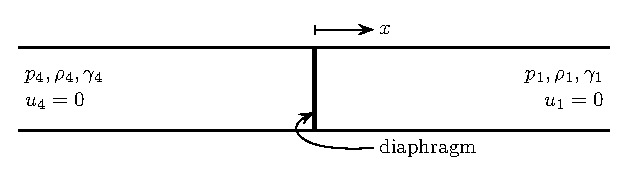
\includegraphics{tube_at_rest.eps}
\caption{Gases are at rest in the tube.}
\label{f:tube_at_rest}
\end{figure}

Consider a one-dimensional tube filled with two gases that are separated by a
diaphragm (see \figurename~\ref{f:tube_at_rest}).  A high-pressure gas is at
the left-hand side, and a low-pressure gas is at the right-hand side.  $p$
denotes the pressure, $\rho$ the mass density, $\gamma$ the ratio of specific
heat, and $u$ the velocity.  The gases is at rest initially ($t = t_0$).
\begin{align}
  p_1 < p_4 , \quad
  \rho_1 < \rho_4, \quad
  u_1 = u_4
\end{align}
The gas at the high-pressure side is called the driving gas, while the gas at
the low-pressure side is called the driven gas.  When the diaphragm is removed,
the driving gas pushes toward the driven gas and the gases around the diaphragm
starts to move to right.  See \figurename~\ref{f:tube_move_right}.

\begin{figure}[h]
\centering
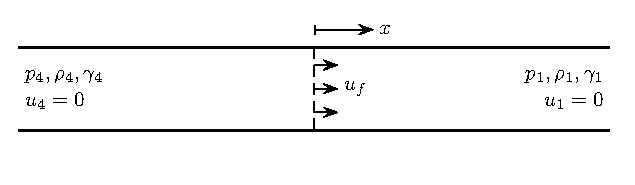
\includegraphics{tube_move_right.eps}
\caption{Gases move to right after the diaphragm disrupts.}
\label{f:tube_move_right}
\end{figure}

Disruption of the diaphragm generates a right-moving normal shock wave and a
left-moving expansion wave.  The flow in the tube looks like
\figurename~\ref{f:tube_zones}.

\begin{figure}[h]
\centering
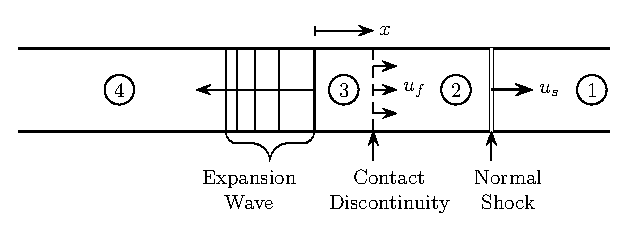
\includegraphics{tube_zones.eps}
\caption{The flow after the diaphragm disrupts in the tube.}
\label{f:tube_zones}
\end{figure}

\end{document}

% vim: set fenc=utf8 ff=unix nobomb et sw=2 ts=2 tw=79:
